\section{Funzioni}

\pgfplotsset{
	standard/.style={
			axis line style = thick,
			trig format = rad,
			enlargelimits,
			axis x line = middle,
			axis y line = middle,
			enlarge x limits = 0.15,
			enlarge y limits = 0.15,
			every axis x label/.style={at{(current axis.right of origin)}, anchor=north west},
			every axis y label/.style={at{(current axis.above origin)}, anchor=south east},
			grid=both
		}
}

\begin{center}
	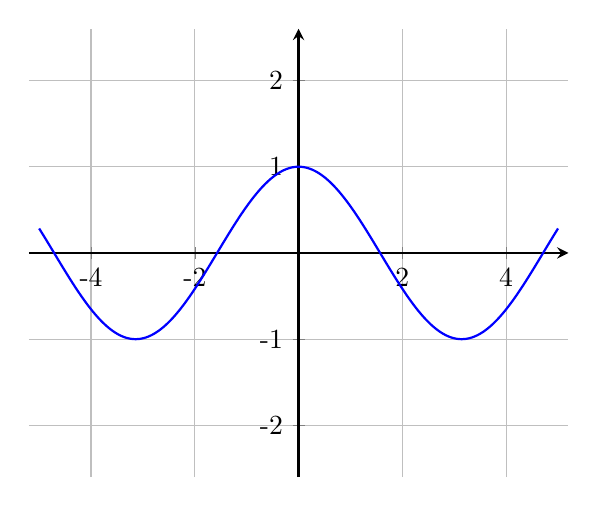
\begin{tikzpicture}
		\begin{axis}[
				standard,
				xtick={-4, -2, 2, 4},
				xticklabels={-4, -2, 2, 4},
				ytick={-2, -1, 1, 2},
				yticklabels={-2, -1, 1, 2},
				samples=1000,
				xmin=-4, xmax=4, ymin=-2, ymax=2
			]

			\addplot[blue, thick]{cos(x)};

		\end{axis}
	\end{tikzpicture}
\end{center}

\begin{center}
	\begin{tikzpicture}
		\begin{axis}[
				standard,
				xtick={-2, -1, 1, 2},
				xticklabels={-2, -1, 1, 2},
				ytick={-2, -1, 1, 2},
				yticklabels={-2, -1, 1, 2},
				samples=1000,
				xmin=-2, xmax=2, ymin=-2, ymax=2
			]
			\node[anchor=center, label=south west: $O$] at (axis cs: 0, 0){};

			\addplot[name path=F, domain={-3:3}, thick, blue] {x^3 + x^2 - x - 0.5};

			\path[name path=xAxis] (axis cs:-1.45, 0) -- (axis cs:0.85, 0);
			\addplot[fill=blue, fill opacity=0.2] fill between [of=F and xAxis, soft clip={domain=-1.45:0.85}];
		\end{axis}
	\end{tikzpicture}
\end{center}